\documentclass[12pt,a4paper]{article}

% ── Packages ──────────────────────────────────────────────────────────────────
\usepackage[margin=2.5cm]{geometry}
\usepackage{amsmath, amssymb}
\usepackage{graphicx}
\usepackage{listings}
\usepackage{xcolor}
\usepackage{booktabs}
\usepackage{hyperref}
\usepackage{caption}
\usepackage{subcaption}
\usepackage{float}
\usepackage{fancyhdr}
\usepackage{titlesec}
\usepackage{enumitem}
\usepackage{mdframed}

% ── Page style ────────────────────────────────────────────────────────────────
\pagestyle{fancy}
\fancyhf{}
\rhead{AM Modulation \& Demodulation}
\lhead{PlutoSDR Laboratory Manual}
\cfoot{\thepage}

% ── Section formatting ────────────────────────────────────────────────────────
\titleformat{\section}{\large\bfseries\color{blue!70!black}}{{\thesection}}{1em}{}[\titlerule]
\titleformat{\subsection}{\normalsize\bfseries\color{blue!50!black}}{\thesubsection}{1em}{}

% ── MATLAB listing style ──────────────────────────────────────────────────────
\definecolor{matlabgreen}{rgb}{0.13,0.55,0.13}
\definecolor{matlabblue}{rgb}{0.0,0.0,0.85}
\definecolor{matlabgray}{rgb}{0.5,0.5,0.5}
\definecolor{codebg}{rgb}{0.97,0.97,0.97}

\lstdefinestyle{matlab}{
  language=Matlab,
  backgroundcolor=\color{codebg},
  basicstyle=\ttfamily\footnotesize,
  keywordstyle=\color{matlabblue}\bfseries,
  commentstyle=\color{matlabgreen}\itshape,
  stringstyle=\color{red!70!black},
  numberstyle=\tiny\color{matlabgray},
  numbers=left,
  numbersep=8pt,
  stepnumber=1,
  frame=single,
  framerule=0.5pt,
  rulecolor=\color{gray!40},
  breaklines=true,
  breakatwhitespace=false,
  tabsize=4,
  showstringspaces=false,
  captionpos=b,
}

% ── Hyperref setup ────────────────────────────────────────────────────────────
\hypersetup{
  colorlinks=true,
  linkcolor=blue!70!black,
  urlcolor=blue,
  citecolor=red!70!black,
}

% ══════════════════════════════════════════════════════════════════════════════
\begin{document}

% ── Title page ────────────────────────────────────────────────────────────────
\begin{titlepage}
  \centering
  \vspace*{2cm}
  {\Huge\bfseries\color{blue!70!black} AM Modulation \& Demodulation\\[0.4em]
   \large Laboratory Manual}\\[1.5cm]
  {\large\itshape Using MATLAB and the ADALM-PlutoSDR}\\[3cm]

  \begin{mdframed}[linecolor=blue!50,linewidth=1.5pt,roundcorner=8pt,backgroundcolor=blue!5]
    \centering\large
    \textbf{Experiment Overview}\\[0.5em]
    This manual covers the end-to-end implementation of\\
    Amplitude Modulation (AM/DSB-LC) using MATLAB and\\
    the ADALM-PlutoSDR software-defined radio platform.
  \end{mdframed}

  \vfill
  {\large Department of Electrical Engineering Department}\\[0.3em]
  {\large\today}
\end{titlepage}

% ── Table of contents ─────────────────────────────────────────────────────────
\tableofcontents
\newpage

% ══════════════════════════════════════════════════════════════════════════════
\section{Introduction}

Amplitude Modulation (AM) is one of the oldest and most fundamental analog
modulation techniques in communication engineering. In AM, the amplitude of a
high-frequency \emph{carrier} signal is varied in proportion to the
\emph{message} (baseband) signal, while the carrier frequency itself remains
constant.

This experiment implements the complete AM modulation and demodulation chain
using MATLAB and the ADALM-PlutoSDR (Pluto Software Defined Radio). The Pluto
SDR provides a low-cost, full-duplex radio platform operating from 70 MHz to
6 GHz, making it an ideal tool for hands-on RF communications experiments.

\subsection{Learning Objectives}

Upon completing this experiment, students should be able to:
\begin{enumerate}[label=\arabic*.]
  \item Derive and implement the mathematical model of DSB-LC AM modulation.
  \item Generate a complex baseband (IQ) signal suitable for SDR transmission.
  \item Transmit and receive an AM signal using the PlutoSDR.
  \item Demodulate an AM signal using envelope detection.
  \item Design and apply a Butterworth low-pass filter to recover the message.
  \item Interpret time-domain and frequency-domain plots of the system.
\end{enumerate}

% ══════════════════════════════════════════════════════════════════════════════
\section{Theoretical Background}

\subsection{AM (DSB-LC) Signal Model}

In Double-Sideband Large Carrier (DSB-LC) AM, the transmitted signal is:

\begin{equation}
  s_{\mathrm{AM}}(t) = A_c\bigl[1 + k_a\, m(t)\bigr]\cos(2\pi f_c t)
  \label{eq:am}
\end{equation}

\noindent where:
\begin{itemize}
  \item $A_c$ — carrier amplitude (normalized to 1 in this experiment),
  \item $k_a$ — amplitude sensitivity (modulation index),
  \item $m(t)$ — normalized message signal $\bigl(|m(t)|\le 1\bigr)$,
  \item $f_c$ — carrier frequency.
\end{itemize}

For a sinusoidal message $m(t) = \cos(2\pi f_m t)$, Equation~\ref{eq:am}
expands to:

\begin{equation}
  s_{\mathrm{AM}}(t) = A_c\cos(2\pi f_c t)
    + \frac{k_a A_c}{2}\cos\bigl[2\pi(f_c+f_m)t\bigr]
    + \frac{k_a A_c}{2}\cos\bigl[2\pi(f_c-f_m)t\bigr]
\end{equation}

This reveals three spectral lines: the carrier at $f_c$ and two sidebands at
$f_c \pm f_m$.

\subsection{Modulation Index}

The modulation index $\mu$ (here $= k_a$ for a single-tone message) determines
the depth of modulation:

\begin{equation}
  \mu = k_a = \frac{A_{\max} - A_{\min}}{A_{\max} + A_{\min}}
\end{equation}

For $\mu < 1$ the signal is under-modulated; $\mu = 1$ gives 100\% modulation;
$\mu > 1$ causes over-modulation (envelope distortion and impossible envelope
detection).  This experiment uses $k_a = 0.8$ (80\% modulation) to ensure
clean envelope detection.

\subsection{Baseband (IQ) Representation}

The PlutoSDR operates on complex baseband signals. The \emph{analytic signal}
(Hilbert transform) of $s_{\mathrm{AM}}(t)$ shifts all energy to positive
frequencies and creates the complex IQ representation:

\begin{equation}
  s_{\mathrm{BB}}(t) = \mathcal{H}\{s_{\mathrm{AM}}(t)\}
    = s_{\mathrm{AM}}(t) + j\,\hat{s}_{\mathrm{AM}}(t)
\end{equation}

\noindent where $\hat{s}_{\mathrm{AM}}(t)$ is the Hilbert transform of
$s_{\mathrm{AM}}(t)$.  The in-phase component $I(t)=\mathrm{Re}\{s_{\mathrm{BB}}\}$
and quadrature component $Q(t)=\mathrm{Im}\{s_{\mathrm{BB}}\}$ are the two
physical channels fed to the SDR DAC.

\subsection{Envelope Detection}

The simplest AM demodulator computes the magnitude of the received IQ signal:

\begin{equation}
  e(t) = \bigl|r_{\mathrm{IQ}}(t)\bigr| = \sqrt{I_r^2(t) + Q_r^2(t)}
\end{equation}

After removing the DC offset (proportional to $A_c$) and normalizing:

\begin{equation}
  \hat{m}(t) = \frac{e(t) - \overline{e}}{\max|e(t) - \overline{e}|}
    \approx m(t)
\end{equation}

A low-pass filter is then applied to suppress residual high-frequency components
introduced by hardware imperfections or channel noise.

\subsection{Butterworth Low-Pass Filter}

The recovered envelope is filtered with a second-order Butterworth IIR filter.
The Butterworth design maximizes the passband flatness.  The transfer function in
the $z$-domain is obtained via the bilinear transform of the analogue prototype.
The normalized cutoff frequency is:

\begin{equation}
  \Omega_n = \frac{f_{\mathrm{cut}}}{f_s/2}, \qquad f_{\mathrm{cut}} = 8\;\text{kHz}
\end{equation}

Zero-phase filtering (\texttt{filtfilt}) is used to eliminate group-delay
distortion.

% ══════════════════════════════════════════════════════════════════════════════
\section{System Parameters}

Table~\ref{tab:params} summarises all key system parameters used in the
experiment.

\begin{table}[H]
  \centering
  \caption{System Parameters}
  \label{tab:params}
  \begin{tabular}{llll}
    \toprule
    \textbf{Parameter} & \textbf{Symbol} & \textbf{Value} & \textbf{Unit} \\
    \midrule
    Sample rate           & $f_s$          & 1\,000\,000  & Sps   \\
    Tx/Rx centre freq.    & $f_{\rm RF}$   & 100          & MHz   \\
    Baseband carrier      & $f_{c1}$       & 100          & kHz   \\
    Message frequency     & $f_m$          & 5            & kHz   \\
    Modulation index      & $k_a$          & 0.8          & ---   \\
    Number of samples     & $N$            & $1024\times16 = 16\,384$ & ---   \\
    Tx gain               & ---            & $-20$        & dBm   \\
    Rx gain               & ---            & 30           & dB    \\
    LPF cutoff            & $f_{\rm cut}$  & 8            & kHz   \\
    Butterworth order     & $n$            & 2            & ---   \\
    \bottomrule
  \end{tabular}
\end{table}

% ══════════════════════════════════════════════════════════════════════════════
\section{Equipment and Software Requirements}

\begin{itemize}
  \item ADALM-PlutoSDR (connected via USB)
  \item MATLAB R2020b or later
  \item \textbf{Communications Toolbox} (for \texttt{sdrtx}, \texttt{sdrrx})
  \item \textbf{Communications Toolbox Support Package for ADALM-PlutoSDR}
  \item Signal Processing Toolbox (for \texttt{butter}, \texttt{filtfilt},
        \texttt{hilbert})
  \item SMA RF cable (loopback Tx $\rightarrow$ Rx) or antenna pair
\end{itemize}

% ══════════════════════════════════════════════════════════════════════════════
\section{MATLAB Implementation}

\subsection{System Block Diagram}

\begin{figure}[H]
  \centering
  % ── Simple block diagram drawn in tikz if available; fallback text ──
  \fbox{\parbox{0.88\linewidth}{\centering\vspace{6pt}
    \textbf{Signal Chain}\\[4pt]
    $m(t)$ \;$\longrightarrow$\; \textbf{AM Modulator}
    \;$\longrightarrow$\; \textbf{Hilbert} (IQ)
    \;$\longrightarrow$\; \textbf{PlutoSDR Tx}
    \;$\xrightarrow{\text{RF}}$\; \textbf{PlutoSDR Rx}\\[4pt]
    \hspace{6.5cm}$\longrightarrow$\; \textbf{Envelope Det.}
    \;$\longrightarrow$\; \textbf{LPF}
    \;$\longrightarrow$\; $\hat{m}(t)$
    \vspace{6pt}
  }}
  \caption{End-to-end AM modulation/demodulation system block diagram.}
  \label{fig:blockdiag}
\end{figure}

\subsection{Complete MATLAB Code}

\begin{lstlisting}[style=matlab, caption={AM Modulation and Demodulation with PlutoSDR}, label={lst:amcode}]
%% ===== AM MODULATION / DEMODULATION WITH PLUTO SDR =====
clear; clc; close all;

%% System Parameters
fs   = 1e6;        % Sample rate (1 MSps)
fc   = 100e6;      % RF centre frequency for Tx/Rx (100 MHz)
fc1  = 100e3;      % Baseband carrier frequency (100 kHz)
fm   = 5e3;        % Message frequency (5 kHz)
ka   = 0.8;        % Amplitude sensitivity (modulation index = 0.8)
N    = 1024*16;    % Number of samples
t    = (0:N-1)'/fs;% Time vector (column)

%% Generate Message Signal (single audio tone)
m_t = cos(2*pi*fm*t);          % Normalized message signal

%% AM Modulation (DSB-LC)
s_am = (1 + ka*m_t) .* cos(2*pi*fc1*t);

%% Normalize for PlutoSDR (peak amplitude <= 1)
s_am_norm = s_am / max(abs(s_am)) * 0.9;

%% Convert to complex baseband via Hilbert transform
s_bb = hilbert(s_am_norm);     % Analytic signal (I + jQ)

%% === TRANSMIT ===
tx = sdrtx('Pluto');
tx.CenterFrequency    = fc;
tx.BasebandSampleRate = fs;
tx.Gain               = -20;   % Reduce gain to avoid saturation
transmitRepeat(tx, s_bb);

%% === RECEIVE ===
rx = sdrrx('Pluto');
rx.CenterFrequency    = fc;
rx.BasebandSampleRate = fs;
rx.GainSource         = 'Manual';
rx.Gain               = 30;
rx.SamplesPerFrame    = N;
rx.OutputDataType     = 'double';

[rx_iq, ~, ~] = rx();

%% === DEMODULATION: Envelope Detection ===
env            = abs(rx_iq);           % Envelope = sqrt(I^2 + Q^2)
env_dc_removed = env - mean(env);      % Remove DC (carrier component)

%% Normalize recovered signal
m_rec = env_dc_removed / max(abs(env_dc_removed));

%% Butterworth Low-Pass Filter Design
fc_msg       = 5e3;          % Message tone (Hz)
fc_cut       = 8e3;          % Cutoff frequency (Hz)
butter_order = 2;            % Filter order

Wn        = fc_cut / (fs/2);           % Normalized cutoff
[b_but, a_but] = butter(butter_order, Wn, 'low');

% Zero-phase filtering (no phase distortion)
m_rec_lp  = filtfilt(b_but, a_but, m_rec);
m_rec_lp  = m_rec_lp / max(abs(m_rec_lp)); % Renormalize

%% === PLOTS ===
figure('Name','AM Modulation Results','NumberTitle','off');

subplot(3,2,1); plot(t(1:500)*1e3, m_t(1:500));
title('Message Signal m(t)');
xlabel('Time (ms)'); ylabel('Amplitude');

subplot(3,2,2); plot(t(1:500)*1e3, real(s_bb(1:500)));
title('AM Signal (Baseband I)'); xlabel('Time (ms)');

subplot(3,2,3); plot(t(1:500)*1e3, real(rx_iq(1:500)));
title('Received IQ Signal'); xlabel('Time (ms)');

subplot(3,2,4); plot(t(1:500)*1e3, m_rec(1:500));
title('Demodulated Signal - Envelope Detection'); xlabel('Time (ms)');

subplot(3,2,5);
NFFT = 4096;
f_ax = (-NFFT/2:NFFT/2-1)*fs/NFFT/1e3;
S_am = 20*log10(abs(fftshift(fft(s_bb,NFFT)))/NFFT);
plot(f_ax, S_am); xlim([-150 150]);
title('AM Baseband Spectrum');
xlabel('Freq (kHz)'); ylabel('Mag (dB)');

subplot(3,2,6);
plot(t(1:500)*1e3, m_rec_lp(1:500), 'b', 'LineWidth', 1.2);
title('Demodulated Signal (LP Filtered)');
xlabel('Time (ms)'); ylabel('Amplitude'); grid on;

release(tx); release(rx);
\end{lstlisting}

% ══════════════════════════════════════════════════════════════════════════════
\section{Step-by-Step Procedure}

\begin{enumerate}[label=\textbf{Step \arabic*.}, leftmargin=*, itemsep=6pt]

  \item \textbf{Hardware Setup.}
        Connect the ADALM-PlutoSDR to the PC via USB.  Connect the Tx SMA port
        to the Rx SMA port using a short coaxial cable (loopback) or use two
        antennas placed in proximity.

  \item \textbf{Install Support Package.}
        In MATLAB, go to \textit{Add-Ons} $\rightarrow$
        \textit{Communications Toolbox Support Package for ADALM-PlutoSDR} and
        follow the installer.

  \item \textbf{Verify Connection.}
        Run \texttt{sdrinfo('Pluto')} in the MATLAB Command Window and confirm
        the device is detected.

  \item \textbf{Set Parameters.}
        Open the script and confirm the parameters in Table~\ref{tab:params}
        match your setup.  Adjust \texttt{tx.Gain} and \texttt{rx.Gain} if
        the received signal is too weak or clipped.

  \item \textbf{Generate and Modulate.}
        The script creates a 5 kHz cosine message $m(t)$ and applies DSB-LC AM
        modulation with $k_a = 0.8$.  The Hilbert transform converts the real AM
        signal to a complex baseband (IQ) signal.

  \item \textbf{Transmit.}
        \texttt{transmitRepeat} continuously streams $s_{\rm BB}$ through the
        PlutoSDR Tx at 100 MHz.

  \item \textbf{Receive.}
        The Rx object captures $N = 16\,384$ complex IQ samples at the same
        centre frequency.

  \item \textbf{Demodulate.}
        Envelope detection via \texttt{abs(rx\_iq)} extracts the signal
        envelope.  The DC offset is removed by subtracting the mean.  A 2nd-order
        Butterworth LPF (cutoff 8 kHz) is applied using \texttt{filtfilt} for
        zero-phase response.

  \item \textbf{Inspect Results.}
        Six subplots are generated (Section~\ref{sec:results}).  Compare the
        recovered signal to the original message $m(t)$.

  \item \textbf{Release Hardware.}
        \texttt{release(tx)} and \texttt{release(rx)} free the SDR resources.

\end{enumerate}

% ══════════════════════════════════════════════════════════════════════════════
\section{Experimental Results and Analysis}
\label{sec:results}

Figure~\ref{fig:results} shows the six output plots generated by the MATLAB
script.  Each subplot is discussed below.

\begin{figure}[H]
  \centering
  % Replace the path below with the actual figure file if embedding the PDF image
  \fbox{\parbox{0.88\linewidth}{\centering\vspace{8pt}
    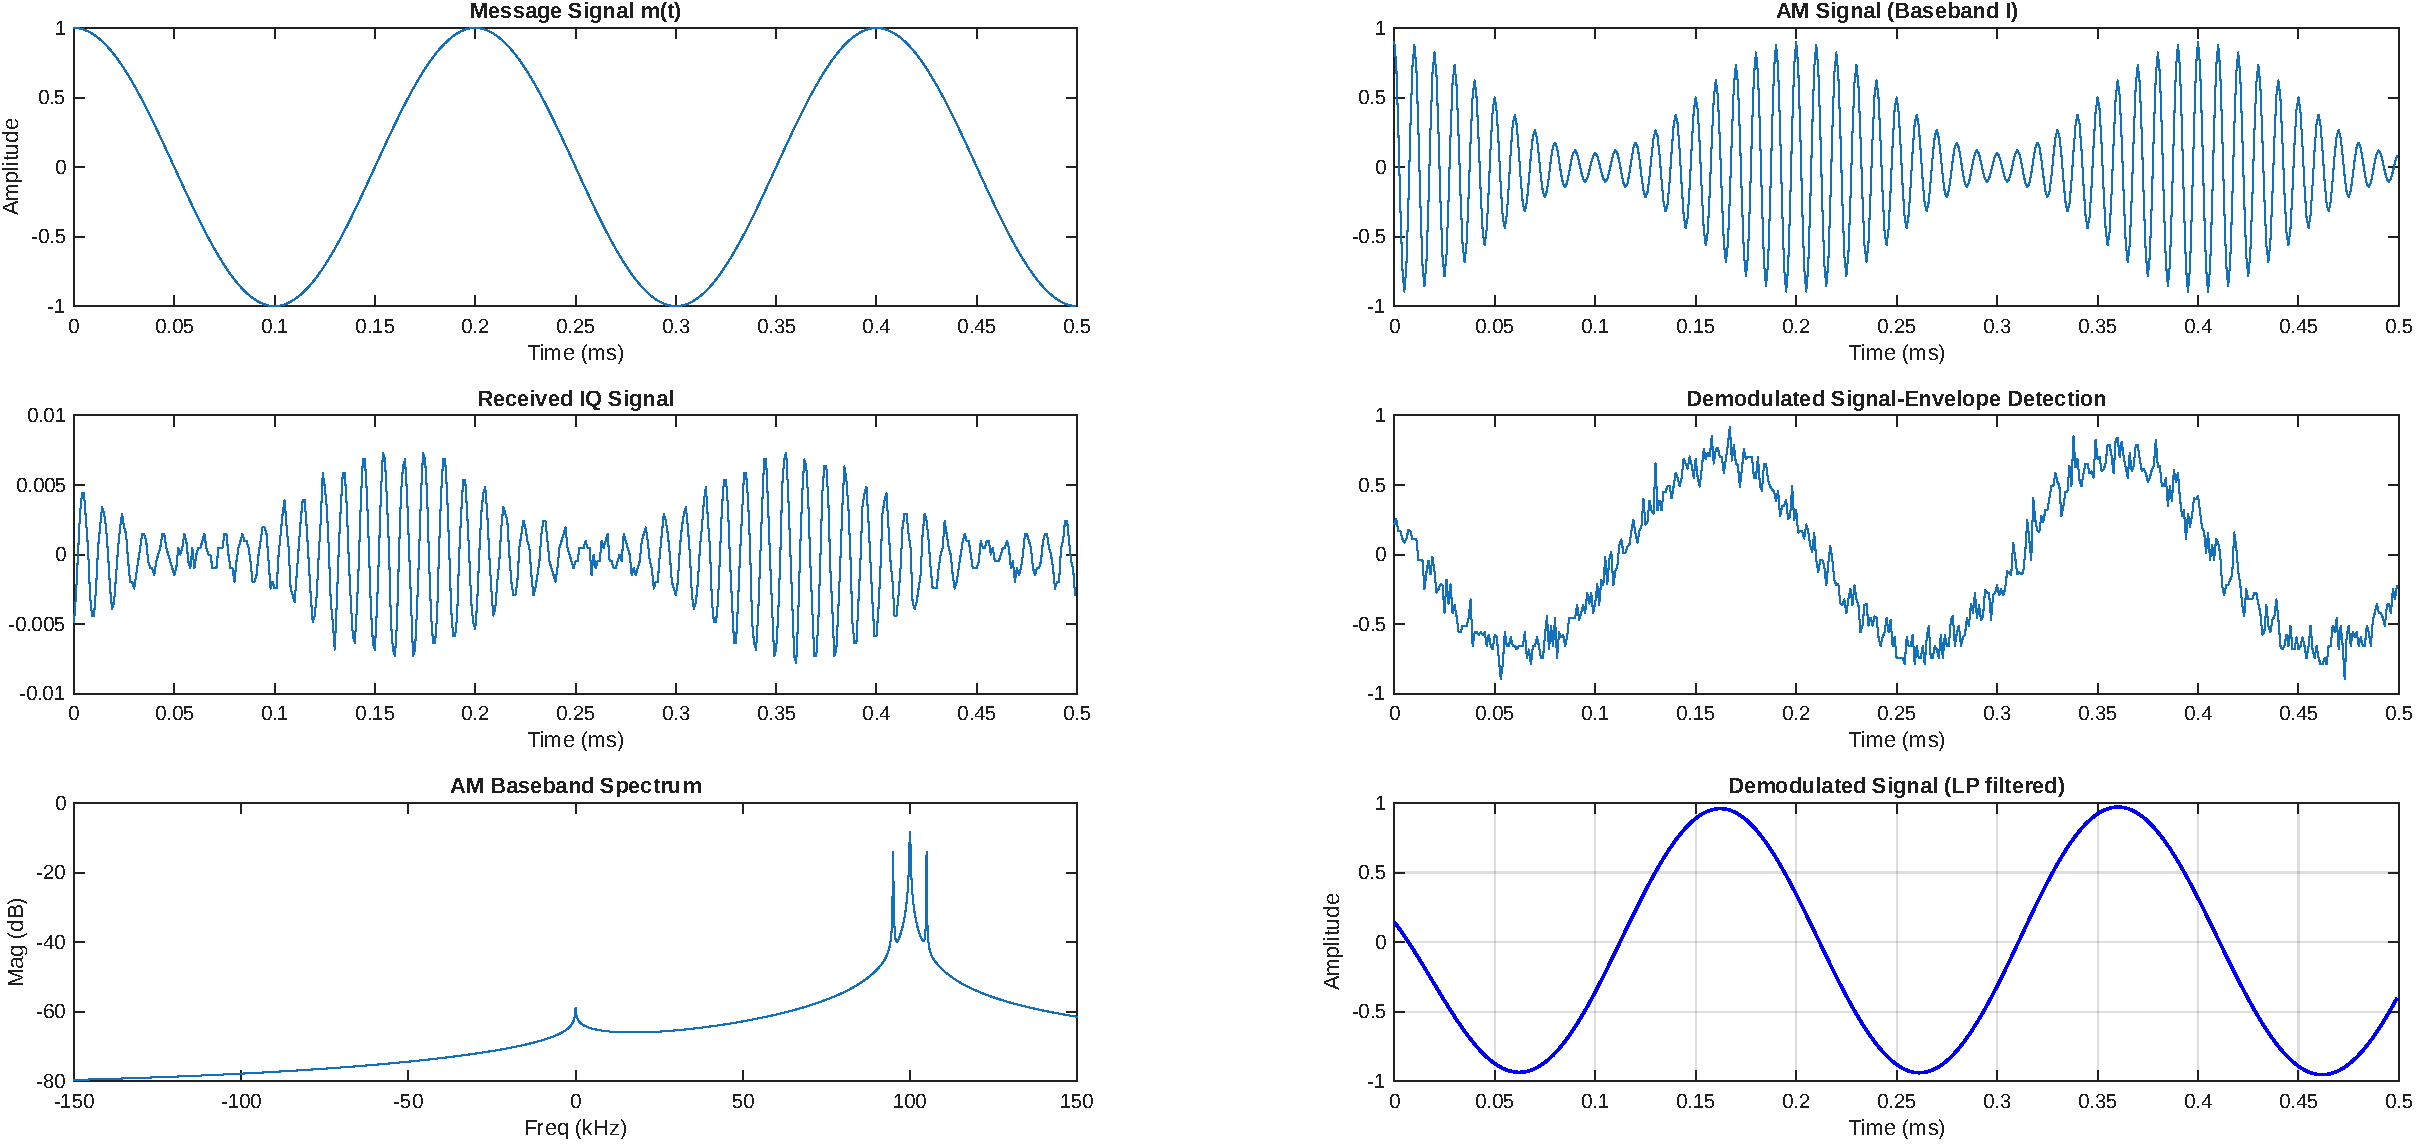
\includegraphics[width=\linewidth]{AM_Modulation_Results.pdf}\\
    \small (output from MATLAB)
    \vspace{8pt}
  }}
  \caption{AM modulation and demodulation results (PlutoSDR loopback).}
  \label{fig:results}
\end{figure}

\subsection{Message Signal $m(t)$ — Subplot 1}

A pure 5 kHz sinusoidal tone of unit amplitude.  It serves as the baseband
information signal.  The time axis spans 0 to 0.5 ms, showing approximately
2.5 cycles of the message.

\subsection{AM Baseband I-Component — Subplot 2}

This is the real part of the analytic (complex baseband) signal $s_{\rm BB}(t)$,
equivalent to the in-phase (I) channel.  The sinusoidal amplitude envelope
varying at $f_m = 5$ kHz is clearly visible on the $f_{c1} = 100$ kHz carrier,
confirming correct DSB-LC modulation with $k_a = 0.8$.

\subsection{Received IQ Signal — Subplot 3}

The signal captured by the PlutoSDR receiver.  The amplitude is significantly
lower ($\approx \pm 0.01$) compared to the transmitted signal, which is expected
due to path loss, the Tx gain of $-20$ dBm, and the hardware RF chain
attenuation.  The waveform shape (AM envelope) is nonetheless preserved.

\subsection{Envelope-Detected Signal — Subplot 4}

After computing $e(t)=|r_{\rm IQ}(t)|$ and removing the DC offset, the
recovered waveform closely resembles the original message $m(t)$.  Minor
distortion and noise are visible, attributable to receiver noise and hardware
non-idealities.

\subsection{AM Baseband Spectrum — Subplot 5}

The power spectral density (in dB) of $s_{\rm BB}$ is plotted over $\pm 150$ kHz.
Three dominant spectral lines are visible:
\begin{itemize}
  \item \textbf{Centre (0 kHz):} residual DC / carrier component.
  \item \textbf{$\pm 100$ kHz:} the baseband carrier at $f_{c1}$.
  \item \textbf{$\pm 95$ and $\pm 105$ kHz:} the two AM sidebands at
        $f_{c1} \pm f_m$.
\end{itemize}

\subsection{Low-Pass Filtered Demodulated Signal — Subplot 6}

Applying the 2nd-order Butterworth LPF (cutoff 8 kHz) with \texttt{filtfilt}
removes residual carrier harmonics and noise while preserving the 5 kHz message.
The resulting waveform is a clean sinusoid closely matching $m(t)$, validating
the complete AM demodulation chain.

% ══════════════════════════════════════════════════════════════════════════════
\section{Key Signal Processing Concepts}

\begin{mdframed}[linecolor=blue!40, linewidth=1pt, roundcorner=6pt,
                  backgroundcolor=blue!3]
\textbf{Hilbert Transform and Analytic Signal}

The \texttt{hilbert()} function in MATLAB returns the \emph{analytic signal},
not simply the Hilbert transform.  The analytic signal
$x_a(t) = x(t) + j\hat{x}(t)$ has a one-sided spectrum (energy only at positive
frequencies), which is the correct format for SDR baseband transmission.
\end{mdframed}

\vspace{8pt}

\begin{mdframed}[linecolor=green!50!black, linewidth=1pt, roundcorner=6pt,
                  backgroundcolor=green!3]
\textbf{Zero-Phase Filtering with \texttt{filtfilt}}

Standard IIR filtering introduces a frequency-dependent group delay.
\texttt{filtfilt} applies the filter \emph{twice} — once forward and once
backward — resulting in zero net phase shift.  This prevents time-domain
distortion of the recovered waveform.
\end{mdframed}

\vspace{8pt}

\begin{mdframed}[linecolor=orange!70!black, linewidth=1pt, roundcorner=6pt,
                  backgroundcolor=orange!3]
\textbf{Gain Selection}

\begin{itemize}
  \item \textbf{Tx Gain $= -20$ dBm:} prevents PlutoSDR DAC saturation and
        reduces self-interference in loopback.
  \item \textbf{Rx Gain $= 30$ dB:} amplifies the weak received signal to a
        usable level.  If clipping occurs, reduce this value.
\end{itemize}
\end{mdframed}

% ══════════════════════════════════════════════════════════════════════════════
\section{Observations and Discussion Questions}

Answer the following questions in your lab report:

\begin{enumerate}[label=\textbf{Q\arabic*.}, leftmargin=*, itemsep=6pt]

  \item Why is the received signal amplitude (Subplot 3) much smaller than the
        transmitted signal (Subplot 2)?  What hardware and propagation factors
        contribute?

  \item What would happen to Subplot 4 if the modulation index were increased
        to $k_a = 1.2$?  Sketch the expected envelope shape and explain.

  \item Explain why \texttt{filtfilt} is preferred over a single \texttt{filter}
        call for this application.

  \item In the spectrum (Subplot 5), identify the carrier and sidebands.
        What is the bandwidth of the transmitted AM signal?  How does it relate
        to the message bandwidth?

  \item How would you modify the code to transmit a speech signal (audio file)
        instead of a single sinusoidal tone?  List the changes required.

  \item If the cutoff frequency of the Butterworth filter were lowered from
        8 kHz to 3 kHz, how would Subplot 6 change?

\end{enumerate}

% ══════════════════════════════════════════════════════════════════════════════
\section{Troubleshooting}

\begin{table}[H]
  \centering
  \caption{Common Issues and Solutions}
  \begin{tabular}{p{4.5cm} p{8.5cm}}
    \toprule
    \textbf{Problem} & \textbf{Solution} \\
    \midrule
    PlutoSDR not detected &
      Run \texttt{sdrinfo('Pluto')} and check USB connection.
      Reinstall the support package driver. \\[4pt]
    Received signal is all zeros &
      Verify Tx/Rx are tuned to the same \texttt{CenterFrequency}.
      Increase \texttt{rx.Gain}. \\[4pt]
    Received signal is clipped / saturated &
      Reduce \texttt{rx.Gain} or \texttt{tx.Gain}. \\[4pt]
    Demodulated signal is noisy &
      Increase \texttt{N} (more samples), lower Butterworth cutoff, or
      improve antenna placement. \\[4pt]
    \texttt{filtfilt} instability & 
      Ensure Wn $\in (0,1)$. Raise the filter cutoff or reduce the order. \\[4pt]
    Phase inversion in $\hat{m}(t)$ &
      Multiply \texttt{m\_rec} by $-1$ if the recovered signal is inverted
      (normal for some channel phases). \\
    \bottomrule
  \end{tabular}
\end{table}

% ══════════════════════════════════════════════════════════════════════════════
\section{Conclusion}

This experiment demonstrated a complete AM (DSB-LC) communication link using
MATLAB and the ADALM-PlutoSDR.  Key outcomes include:

\begin{itemize}
  \item Successful generation of a DSB-LC AM signal with modulation index
        $k_a = 0.8$ and verification of its spectrum showing a carrier and two
        sidebands.
  \item Conversion to complex baseband (IQ) format using the Hilbert transform
        for PlutoSDR transmission at 100 MHz.
  \item Over-the-air (loopback) reception and envelope detection
        of the received IQ signal.
  \item Clean message recovery using DC removal and a 2nd-order Butterworth
        low-pass filter with zero-phase implementation (\texttt{filtfilt}).
\end{itemize}

The experiment confirms that envelope detection is an effective and simple
demodulation method for AM signals with modulation index $< 1$, and that
software-defined radio platforms like the PlutoSDR provide an accessible
environment for implementing real RF communication systems.

% ══════════════════════════════════════════════════════════════════════════════
\section*{References}
\addcontentsline{toc}{section}{References}

\begin{enumerate}[label={[\arabic*]}]
  \item Haykin, S., \textit{Communication Systems}, 4th ed., Wiley, 2001.
  \item Proakis, J. G. \& Salehi, M., \textit{Communication Systems Engineering},
        2nd ed., Prentice Hall, 2002.
  \item Analog Devices, \textit{ADALM-PlutoSDR Learning Module},
        \url{https://wiki.analog.com/university/tools/pluto}, 2023.
  \item MathWorks, \textit{Communications Toolbox — ADALM-PlutoSDR Support},
        \url{https://www.mathworks.com/hardware-support/pluto.html}, 2024.
  \item Oppenheim, A. V. \& Schafer, R. W., \textit{Discrete-Time Signal
        Processing}, 3rd ed., Prentice Hall, 2010.
\end{enumerate}

\end{document}
